% Generated by code/ch08_hierarchy.py -- do not edit by hand.
\definecolor{qocA}{rgb}{0.00,0.45,0.70}
\definecolor{qocB}{rgb}{0.90,0.60,0.00}
\definecolor{qocC}{rgb}{0.00,0.62,0.45}
\definecolor{qocD}{rgb}{0.80,0.40,0.00}
\definecolor{qocE}{rgb}{0.80,0.60,0.70}
\definecolor{qocF}{rgb}{0.35,0.70,0.90}
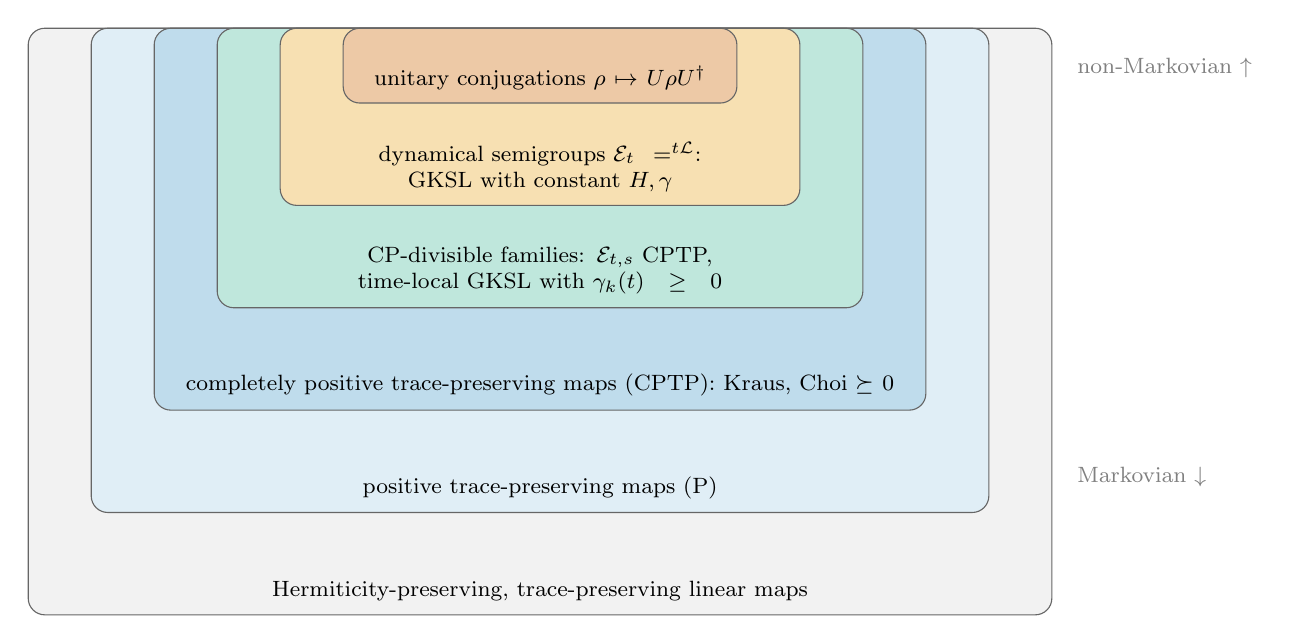
\begin{tikzpicture}[]
\draw[rounded corners=6pt, fill=gray!10, draw=black!60] (-6.50,-7.45) rectangle (6.50,0);
\node[anchor=south, font=\footnotesize, text width=12.60cm, align=center] at (0,-7.40) {Hermiticity-preserving, trace-preserving linear maps};
\draw[rounded corners=6pt, fill=qocA!12, draw=black!60] (-5.70,-6.15) rectangle (5.70,0);
\node[anchor=south, font=\footnotesize, text width=11.00cm, align=center] at (0,-6.10) {positive trace-preserving maps (P)};
\draw[rounded corners=6pt, fill=qocA!25, draw=black!60] (-4.90,-4.85) rectangle (4.90,0);
\node[anchor=south, font=\footnotesize, text width=9.40cm, align=center] at (0,-4.80) {completely positive trace-preserving maps (CPTP): Kraus, Choi $\succeq 0$};
\draw[rounded corners=6pt, fill=qocC!25, draw=black!60] (-4.10,-3.55) rectangle (4.10,0);
\node[anchor=south, font=\footnotesize, text width=7.80cm, align=center] at (0,-3.50) {CP-divisible families: $\mathcal{E}_{t,s}$ CPTP, time-local GKSL with $\gamma_k(t)\ge 0$};
\draw[rounded corners=6pt, fill=qocB!30, draw=black!60] (-3.30,-2.25) rectangle (3.30,0);
\node[anchor=south, font=\footnotesize, text width=6.20cm, align=center] at (0,-2.20) {dynamical semigroups $\mathcal{E}_t=\ee^{t\mathcal{L}}$: GKSL with constant $H,\gamma$};
\draw[rounded corners=6pt, fill=qocD!35, draw=black!60] (-2.50,-0.95) rectangle (2.50,0);
\node[anchor=south, font=\footnotesize, text width=4.60cm, align=center] at (0,-0.90) {unitary conjugations $\rho\mapsto U\rho U^\dagger$};
\node[anchor=west, font=\footnotesize, gray] at (6.70,-0.5) {non-Markovian $\uparrow$};
\node[anchor=west, font=\footnotesize, gray] at (6.70,-5.70) {Markovian $\downarrow$};
\end{tikzpicture}
